%DO NOT MESS AROUND WITH THE CODE ON THIS PAGE UNLESS YOU %REALLY KNOW WHAT YOU ARE DOING
\chapter*{Gannt Chart}
\addcontentsline{toc}{chapter}{Gannt Chart}
\noindent  Gantt chart is a visual view of tasks scheduled over time. Figure 4 shows a Gantt chart on which you can see the start date of the project, what the project tasks are, who is working on each task, when tasks start and finish, how long each task will take, how tasks group together, overlap and link with each other and the finish date of the project. The critical paths are shown in red colour while the non-critical paths are shown in blue.

\begin{figure}[h]
\centering
\subfloat{
  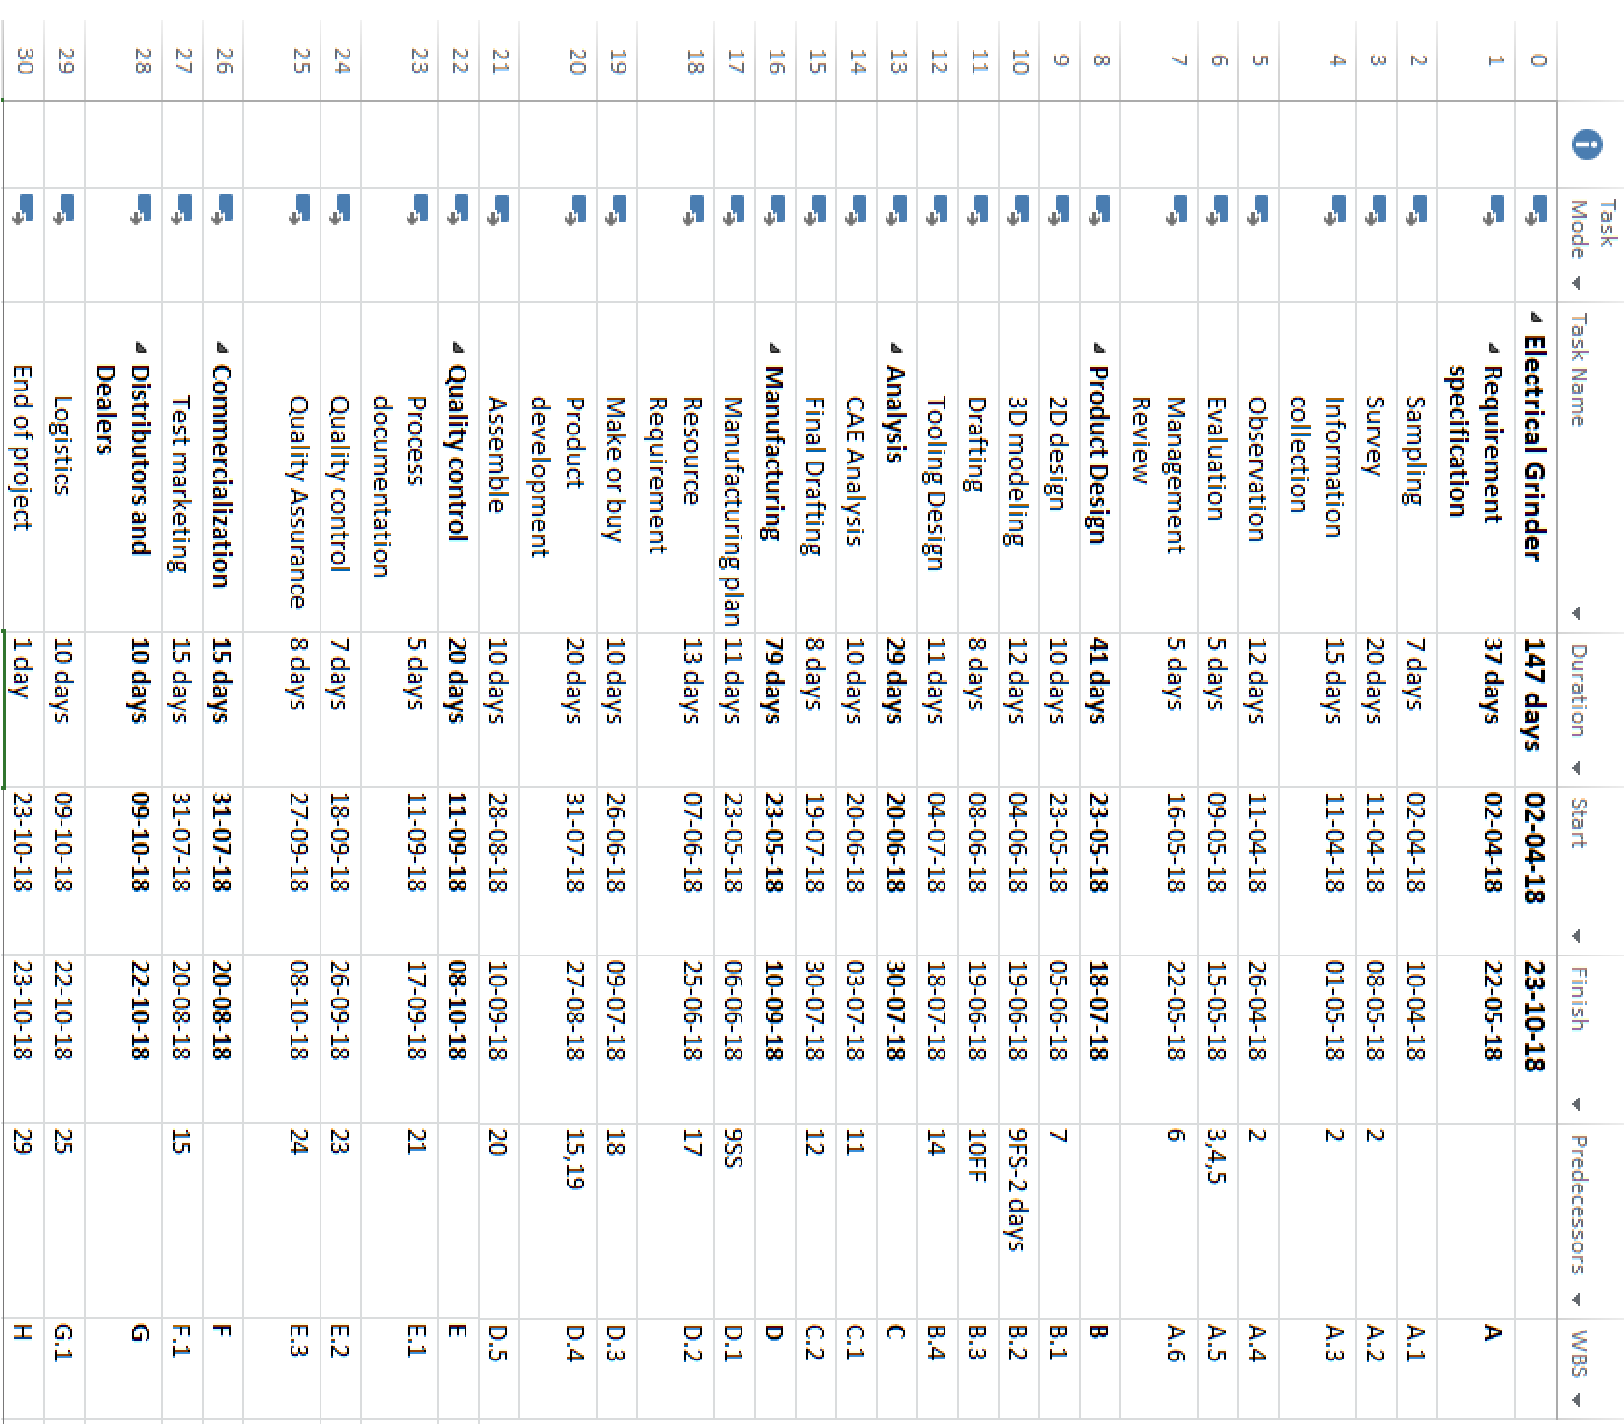
\includegraphics[height=9cm, width=15.5cm]{gannt1.png}
}
\newline
\subfloat {
  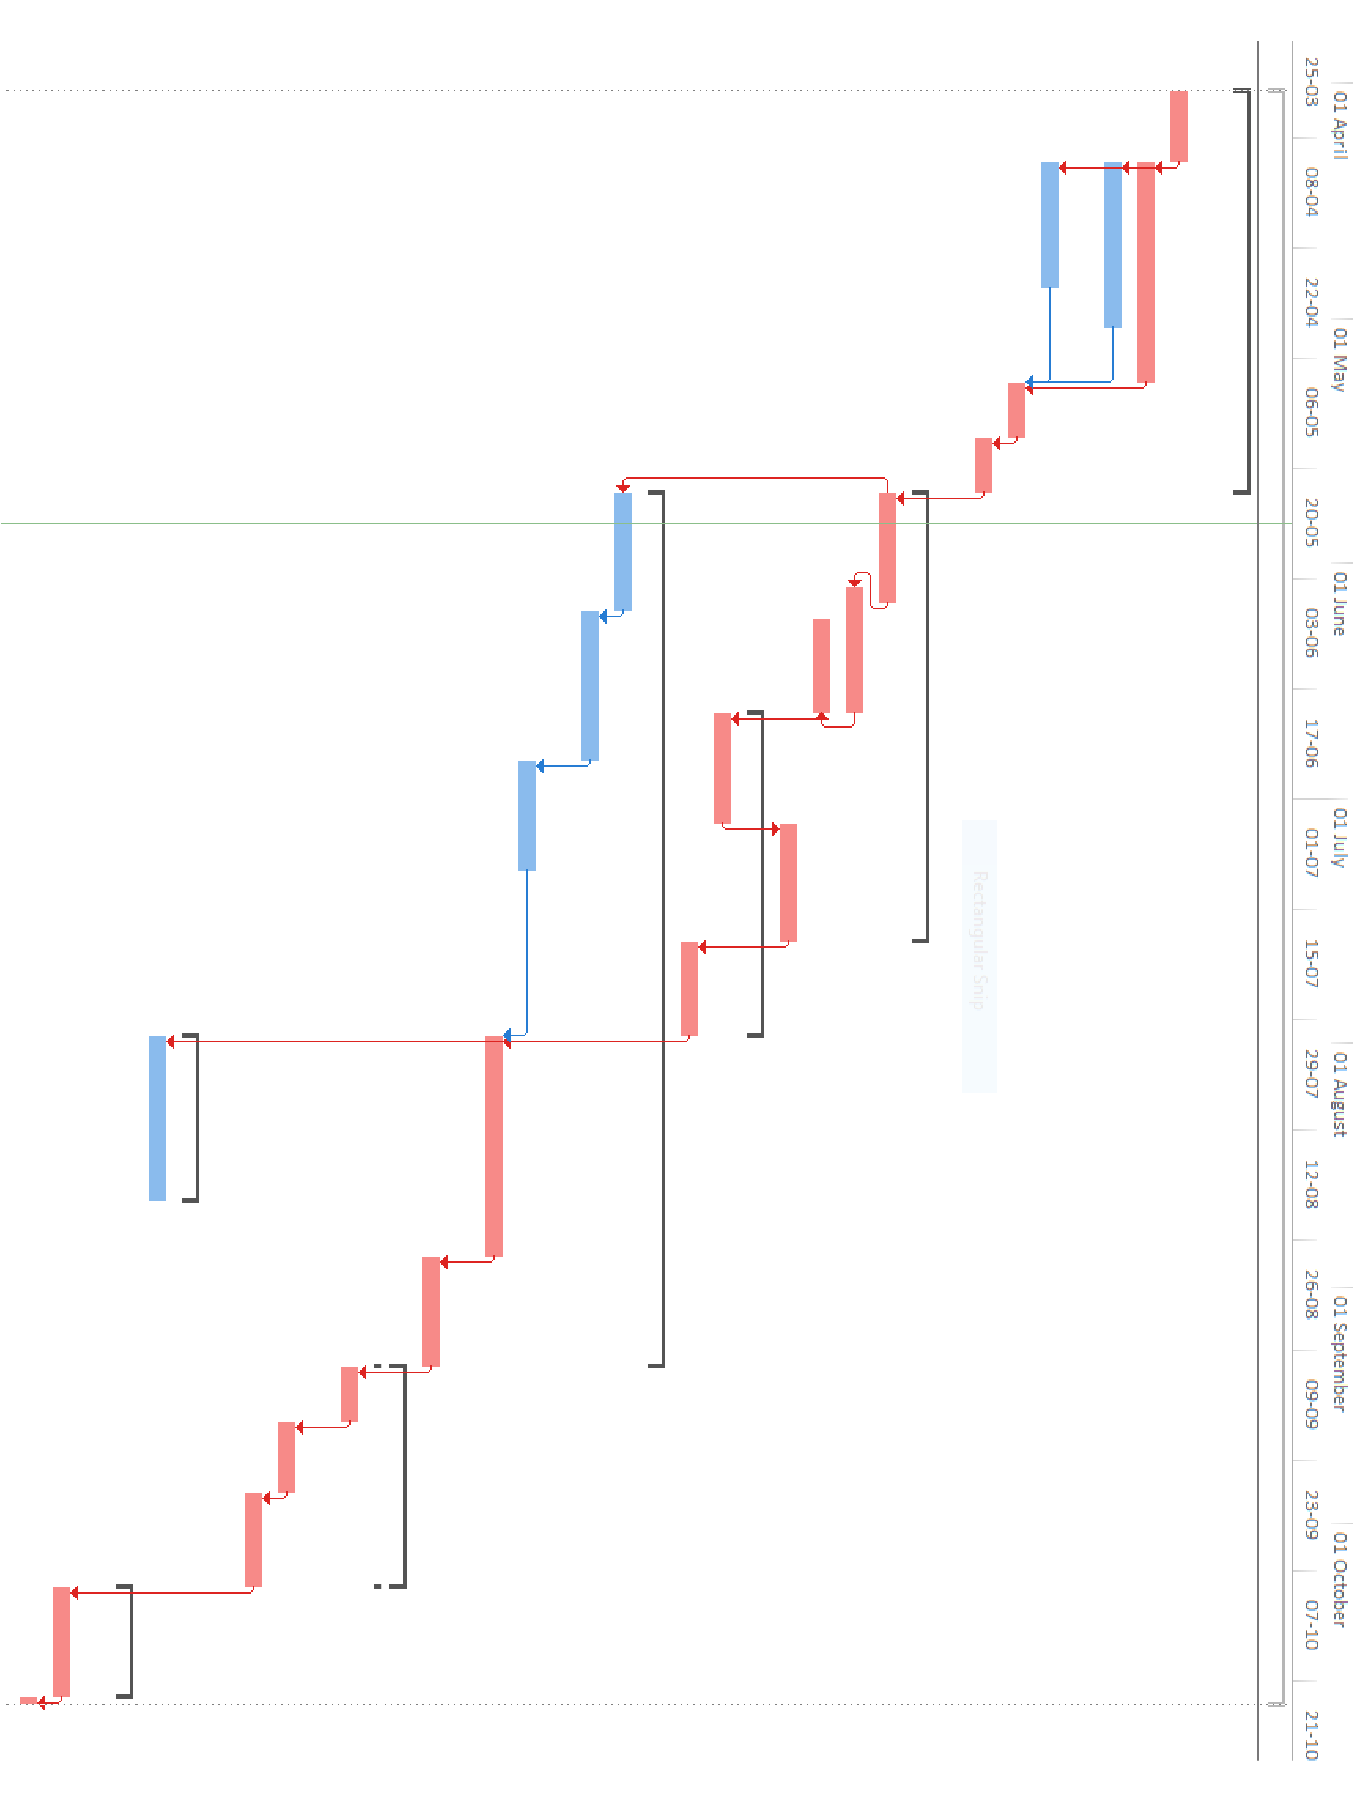
\includegraphics[height=10cm, width=14cm]{gannt2.png}
}
\caption{Gannt Chart }
\end{figure}
